\documentclass[12pt,a4paper]{article}

\usepackage{graphicx}
\usepackage{booktabs}
\usepackage{amsmath}
\usepackage{url}

\graphicspath{{figures/}{../resultsAct3/}}

\begin{document}

\title{\LARGE Parallel Matrix Multiplication using OpenMP and SIMD
Vectorization\\[0.5em]
\normalsize\normalfont Individual Assignment 3 --- Report}
\author{Carlos Montesdeoca Vega\\[8pt]
\texttt{repository:}\\[2pt]
\small\texttt{https://github.com/CarlosMontesdeoca21/BasicMatrixMultiplication}}
\date{October 28, 2026}

\maketitle

\begin{abstract}
This report investigates how the number of threads affects the performance of
a dense matrix multiplication implementation in shared memory, and under what
conditions parallel execution becomes beneficial. We compare a sequential
baseline (classic i-j-k triple loop in C, double precision) against an OpenMP
parallelization of the same kernel over matrix rows, using thread counts
$p \in \{1, 2, 4, 8, 16, 22, 28\}$ on a hybrid 16-core/22-thread Intel Core
Ultra 7 155H. Inputs are deterministic shared matrices up to $n = 1000$;
each configuration is measured 5 times after 2 warm-ups with a
monotonic microsecond-resolution timer, reporting medians and interquartile
ranges. Speedup saturates at $S(p) \approx 5.45$ for $p \geq 16$, with
efficiency dropping from $1.04$ ($p=2$) to $0.25$ ($p=22$); running OpenMP
with a single thread stays within $1.4\%$ of the sequential baseline. As an
optional extension, a sequential i-k-j variant is evaluated under three
compiler configurations: the loop reorder alone reduces the $n=1000$ time
from $858$ ms to $288$ ms, auto-vectorization with \texttt{-O3} reaches
$186$ ms, and \texttt{-march=native} reaches $157$ ms --- comparable to the
16-thread unvectorized parallel run. Conclusions are limited to the tested
hardware, inputs and configurations.
\end{abstract}

\section{Introduction}
\label{sec:intro}

Matrix multiplication is a fundamental operation in scientific computing and
data analytics. Its classical algorithm has cubic time complexity
($O(n^3)$) and poor cache behavior, making it computationally expensive.
The goal of this work is to evaluate the performance improvement obtained
through parallelism in shared memory, and to answer a focused research
question: how does the thread count affect the execution time of an OpenMP
implementation compared with its sequential baseline, and where does the
speedup saturate?

We implement and compare three approaches:
\begin{itemize}
\item Sequential algorithm (classic i-j-k triple loop in C, double
precision);
\item Parallel execution using OpenMP (the same i-j-k kernel, parallelized
over the rows of the result matrix);
\item Sequential i-k-j variant (same arithmetic work and storage, only the
loop order changes, so the innermost loop becomes a vectorizable rank-1
row update).
\end{itemize}

All experiments use the same input matrices per configuration, a documented
measurement protocol with warm-up runs and repetitions, and robust
statistics (median and interquartile range).

\section{Code and organization}
\label{sec:code}

The project repository includes a structured hierarchy with implementations
under the \texttt{Activity3/code} folder alongside management scripts:
\begin{itemize}
\item \textbf{C benchmark (\texttt{benchmark\_omp.c}):} Contains the three
kernels (\texttt{Sequential} i-j-k, \texttt{OpenMP} with
\texttt{\#pragma omp parallel for} over rows, and \texttt{Sequential\_ikj}
for the SIMD study), plus a CSV loader, checksum validation and a memory
metric based on the Windows process API (\texttt{psapi}). The OpenMP kernel
uses \texttt{num\_threads($p$)} and \texttt{schedule(static)}; each row of
the result matrix is written by exactly one thread.
\item \textbf{Python automation scripts:} \texttt{generate\_inputsAct3.py}
creates the deterministic input matrices (seed 42, sizes
$n \in \{10, 100, 250, 500, 1000\}$), \texttt{validate\_act3.py} checks the
sequential result against NumPy, \texttt{merge\_results\_act3.py} computes
medians, IQR, speedup and efficiency, and \texttt{plot\_results\_act3.py}
exports the performance charts.
\item \textbf{Data artifacts:} Raw measurements are stored as CSV files in
\texttt{Activity3/data/} (generated locally, not tracked); consolidated
tables, figures and the compiler vectorization report live in
\texttt{Activity3/resultsAct3/} (tracked).
\item \textbf{Report:} The source of this document is
\texttt{Activity3/report/Report\_assigment3.tex} (LaTeX).
\end{itemize}

Production kernel logic is separated from benchmarking and analysis
scripts, and all matrix sizes and thread counts are fully parameterized via
command-line flags.

\section{Experimental methodology}
\label{sec:method}

\begin{itemize}
\item \textbf{Measurement:} Execution time was measured with
\texttt{QueryPerformanceCounter} (monotonic, $\approx$100 ns resolution) and
converted to milliseconds. Only the multiplication kernel is timed; matrix
loading and allocation are outside the timed region. Memory consumption was
tracked with \texttt{GetProcessMemoryInfo} (process working set, KB). The
OpenMP API \texttt{omp\_get\_wtime()} was rejected because in libgomp on
Windows it only resolves about 1 ms, which quantizes the smaller sizes.
\item \textbf{Warm-up phase \& repetitions:} A fixed warm-up phase
(2 rounds) was executed prior to recording official metrics, and its samples
were excluded from the reported statistics. Following the warm-up, 5
official consecutive repetitions were executed per configuration to capture
statistical variance. The reported statistic is the median of the 5 samples,
with the interquartile range (IQR) as variability measure.
\item \textbf{Performance metrics:} Let $T_{\mathrm{seq}}(n)$ be the time of
the sequential baseline and $T_p(n)$ the parallel time for the same input
with $p$ threads. The speedup and efficiency are
$S(p) = T_{\mathrm{seq}}(n) / T_p(n)$ and $E(p) = S(p) / p$.
\item \textbf{Correctness validation:} Correctness was rigorously validated
by computing a checksum of the resulting matrix and comparing it against the
sequential reference after every parallel configuration (relative tolerance
$10^{-6}$). Additionally, the sequential result for $n = 10$ matches NumPy's
\texttt{A @ B} with a maximum absolute difference of $4.9 \times 10^{-7}$
(absolute tolerance $10^{-6}$). The elementwise difference between
sequential and parallel results is exactly zero, because both kernels
perform the same operation in the same order for every element. All
validations passed.
\item \textbf{Environment:} All experiments were executed on a machine
with: CPU Intel Core Ultra 7 155H (Meteor Lake) --- 6 P-cores + 8 E-cores +
2 low-power E-cores = 16 physical cores / 22 hardware threads, P-cores up to
4.8 GHz; RAM 32 GB; OS Windows 11; compiler gcc 16.2.0 (MSYS2) with flags
\texttt{-O3 -fopenmp}. Python 3.12 was used for input generation and
analysis (numpy, pandas, matplotlib).
\item \textbf{Thread configuration:} The thread counts tested were
$p \in \{1, 2, 4, 8, 16, 22, 28\}$: $p = 22$ matches the number of hardware
contexts and $p = 28$ deliberately oversubscribes the machine (labelled as
such in the results). Explicit thread affinity
(\texttt{OMP\_PROC\_BIND}/\texttt{OMP\_PLACES}) could not be enforced,
because libgomp ignores it on Windows; the OS scheduler placed the workers.
\item \textbf{Budgets:} The declared time and memory budgets were 5 minutes
and 4 GB per multiplication; they were never reached (the largest observed
time was 1.19 s).
\end{itemize}

\section{Data and statistics}
\label{sec:data}

The data extracted from the consolidated benchmarking CSVs are summarized
below. For each configuration (matrix size $n$ and thread count $p$), the
median execution time, the interquartile range (IQR) variability, the
speedup and the efficiency are reported to ensure robust statistical
evaluation.

\subsection{Numerical summary}
\label{sec:numsummary}

Table~\ref{tab:sweep} reports the full thread sweep for the largest tested
size ($n = 1000$), including the sequential baseline and the OpenMP version
with a single thread to expose the framework overhead.
Table~\ref{tab:cross} consolidates the speedup across problem sizes.

\begin{table}[h]
\centering
\caption{Thread sweep for $n = 1000$: median time (IQR $< 2\%$ of the
median), speedup and efficiency.}
\label{tab:sweep}
\begin{tabular}{@{}lcccc@{}}
\toprule
Config & $T_p$ (ms) & IQR (ms) & $S(p)$ & $E(p)$ \\
\midrule
Sequential & 858.2 & 31.9 & --- & --- \\
OpenMP $p=1$ & 846.6 & 7.7 & 1.01 & 1.01 \\
OpenMP $p=2$ & 414.4 & 8.7 & 2.07 & 1.04 \\
OpenMP $p=4$ & 239.2 & 16.9 & 3.59 & 0.90 \\
OpenMP $p=8$ & 177.5 & 5.4 & 4.83 & 0.60 \\
OpenMP $p=16$ & 157.7 & 3.3 & 5.44 & 0.34 \\
OpenMP $p=22$ & 157.4 & 5.3 & 5.45 & 0.25 \\
OpenMP $p=28$ & 158.5 & 1.9 & 5.41 & 0.19 \\
\bottomrule
\end{tabular}
\end{table}

\begin{table}[h]
\centering
\caption{Speedup $S(p)$ by problem size (median times).}
\label{tab:cross}
\begin{tabular}{@{}lcccccc@{}}
\toprule
$n$ & $p=2$ & $p=4$ & $p=8$ & $p=16$ & $p=22$ & $p=28$ \\
\midrule
250 & 2.10 & 2.73 & 2.69 & 4.01 & 4.23 & 4.52 \\
500 & 2.14 & 3.53 & 4.73 & 5.70 & 5.77 & 5.73 \\
1000 & 2.07 & 3.59 & 4.83 & 5.44 & 5.45 & 5.41 \\
\bottomrule
\end{tabular}
\end{table}

\textbf{Note on data aggregation and trends:} The values reported above
correspond to the median times and memory footprints extracted across
multiple official repetitions, effectively mitigating the influence of
isolated system outliers. The OpenMP version with a single thread is within
1.4\% of the plain sequential baseline, so the framework overhead is
negligible at this granularity. For the smallest parallel sizes
($n = 250$), the speedup curve is noisy: the runtime is only a few
milliseconds, so thread-management costs and measurement quantization are a
sizeable fraction of the total. A mild superlinearity is observed at $p = 2$
($S = 2.07$), most plausibly a turbo-frequency regime effect, which is
reported as observed rather than attributed to the measurement. The process
working set is essentially constant across thread counts
($\approx$30.5 MB for $n = 1000$: the three matrices account for about
24 MB, plus the runtime and per-thread stacks, which grow slightly with
$p$).

\subsection{Graphical analysis and plots}
\label{sec:plots}

To visually evaluate the scaling behavior of the parallel implementation and
the effect of SIMD vectorization, comparative execution time, speedup and
efficiency plots were automatically generated from the benchmark data.

\subsubsection{Execution Time Analysis}
\label{sec:timetables}

\begin{figure}[h]
\centering
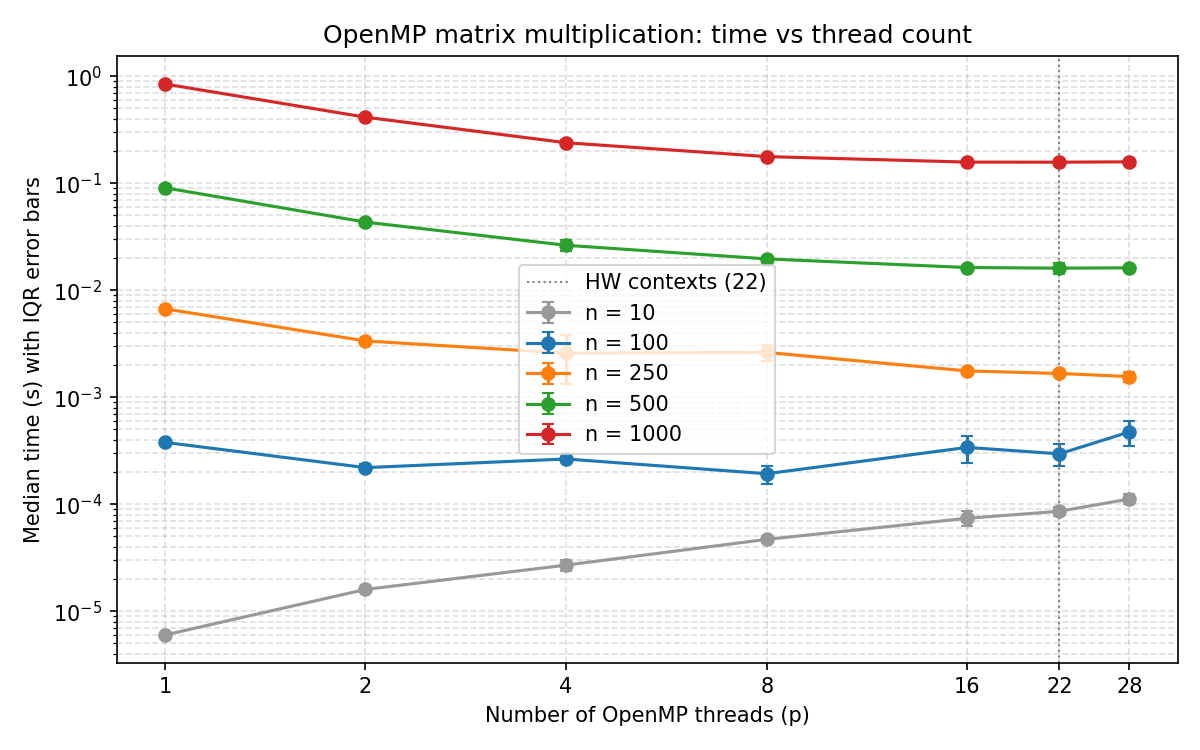
\includegraphics[width=0.9\textwidth]{plot_time_vs_threads_act3.png}
\caption{Execution time (ms, log scale) vs.\ thread count for
$n \in \{250, 500, 1000\}$, with IQR error bars. The dotted line marks the
22 hardware contexts.}
\label{fig:time-threads}
\end{figure}

\begin{figure}[h]
\centering
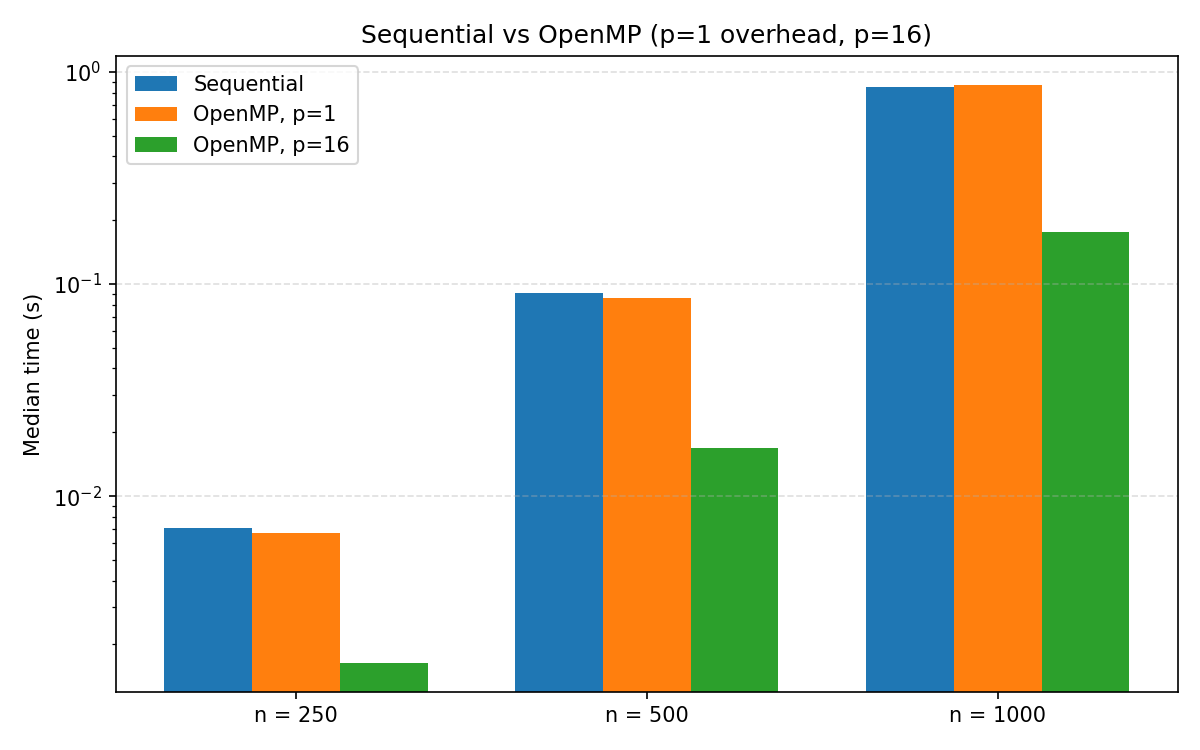
\includegraphics[width=0.9\textwidth]{plot_seq_vs_omp_act3.png}
\caption{Execution time (ms, log scale) vs.\ matrix size: sequential
baseline, OpenMP with $p=1$ (framework overhead) and OpenMP with $p=16$.}
\label{fig:time-size}
\end{figure}

\textbf{Analysis:} As observed in Figure~\ref{fig:time-threads}, execution
time drops steeply as threads are added and then flattens: for $n = 1000$
the time falls from 858 ms (sequential) to 178 ms at $p = 8$ and to about
157 ms at $p = 16$, after which the curve is essentially flat. Small
problems ($n \leq 100$, not plotted) are dominated by thread management:
their time actually increases with $p$, because the computation is shorter
than the cost of creating and joining the thread team.
Figure~\ref{fig:time-size} shows the same data per matrix size: the OpenMP
version at $p = 16$ is about $4.8$--$5.7\times$ faster than the sequential
baseline for $n \in \{250, 500, 1000\}$, while at $p = 1$ it matches it.

\subsubsection{Speedup Analysis}
\label{sec:speedupfig}

\begin{figure}[h]
\centering
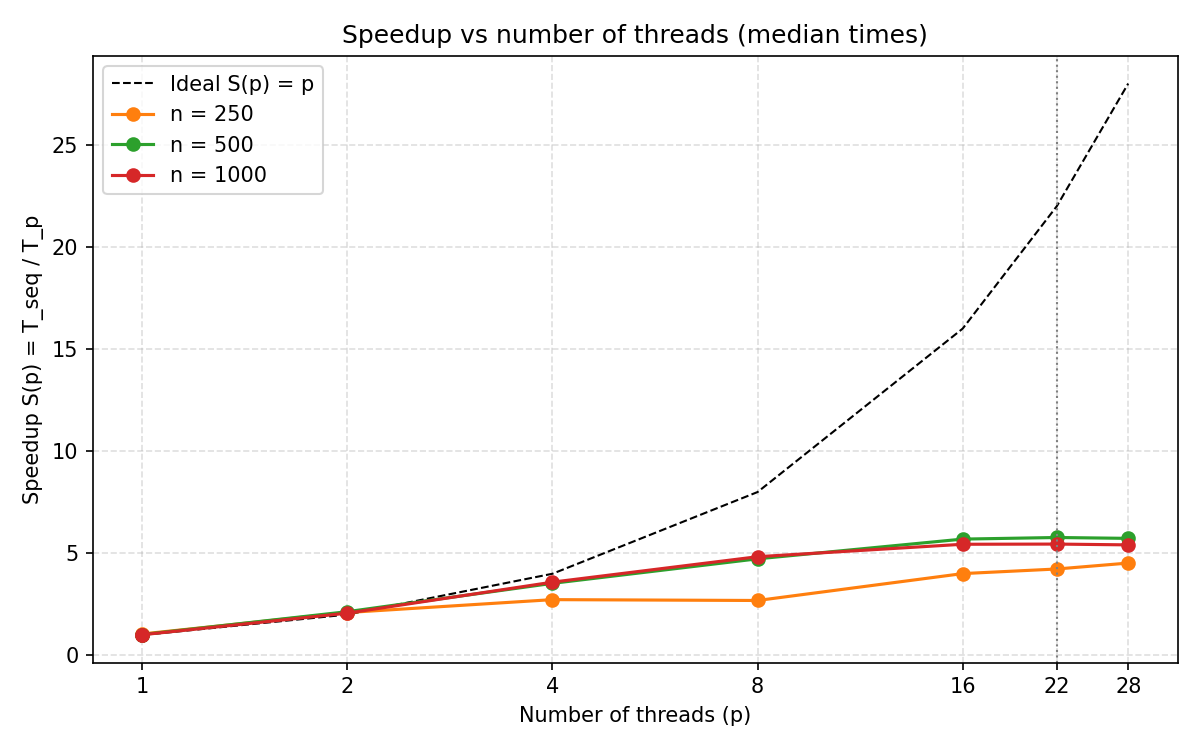
\includegraphics[width=0.9\textwidth]{plot_speedup_vs_threads_act3.png}
\caption{Speedup $S(p) = T_{\mathrm{seq}}/T_p$ (median times) vs.\ thread
count for $n \in \{250, 500, 1000\}$, against the ideal line $S(p) = p$.}
\label{fig:speedup}
\end{figure}

\textbf{Analysis:} Figure~\ref{fig:speedup} plots the speedup against the
ideal linear line. All curves bend away from the ideal early: larger
problems scale better (more computation per unit of thread management), and
$n = 500$ slightly outperforms $n = 1000$ at high thread counts, which is
consistent with memory-bandwidth sharing among more concurrent workers. The
maximum observed speedup is $S(22) = 5.45$ for $n = 1000$
(Table~\ref{tab:sweep}).

\subsubsection{Parallel Efficiency Analysis}
\label{sec:efffig}

\begin{figure}[h]
\centering
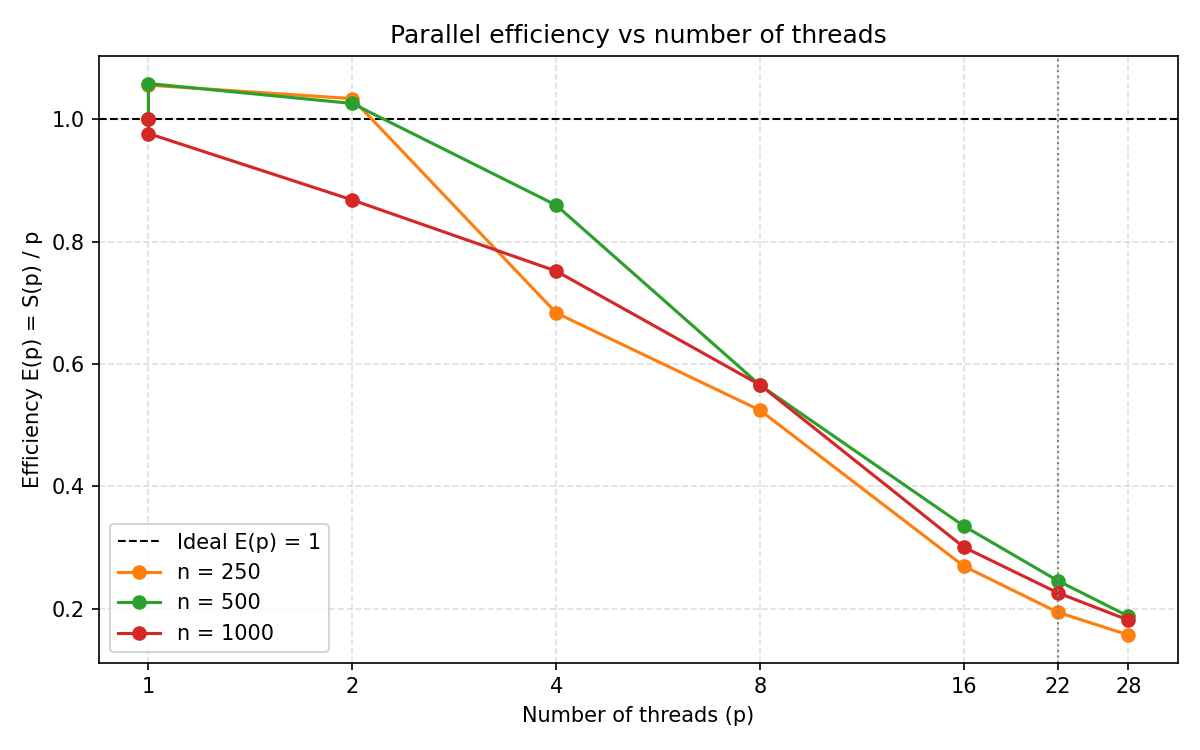
\includegraphics[width=0.9\textwidth]{plot_efficiency_vs_threads_act3.png}
\caption{Parallel execution efficiency $E(p) = S(p)/p$ relative to the
number of threads.}
\label{fig:efficiency}
\end{figure}

\textbf{Analysis:} As presented in Figure~\ref{fig:efficiency}, efficiency
stays close to 1 up to $p = 2$--$4$ and decays as the speedup saturates: at
the maximum observed speedup ($p = 22$, $n = 1000$) only about a quarter of
the theoretical parallel capacity is used, and at $p = 28$
(oversubscription) it falls below 20\%.

\subsubsection{SIMD Vectorization Study}
\label{sec:simd}

\begin{table}[h]
\centering
\caption{SIMD study: median time (ms) of the sequential kernels.}
\label{tab:simd}
\begin{tabular}{@{}lccc@{}}
\toprule
Build & $n=250$ & $n=500$ & $n=1000$ \\
\midrule
i-j-k, \texttt{-O3} & 7.06 & 92.90 & 858.18 \\
i-k-j, \texttt{-O3 -fno-tree-vectorize} & 4.13 & 32.92 & 288.28 \\
i-k-j, \texttt{-O3} & 2.56 & 19.81 & 186.16 \\
i-k-j, \texttt{-O3 -march=native} & 1.80 & 14.58 & 156.85 \\
\bottomrule
\end{tabular}
\end{table}

\begin{figure}[h]
\centering
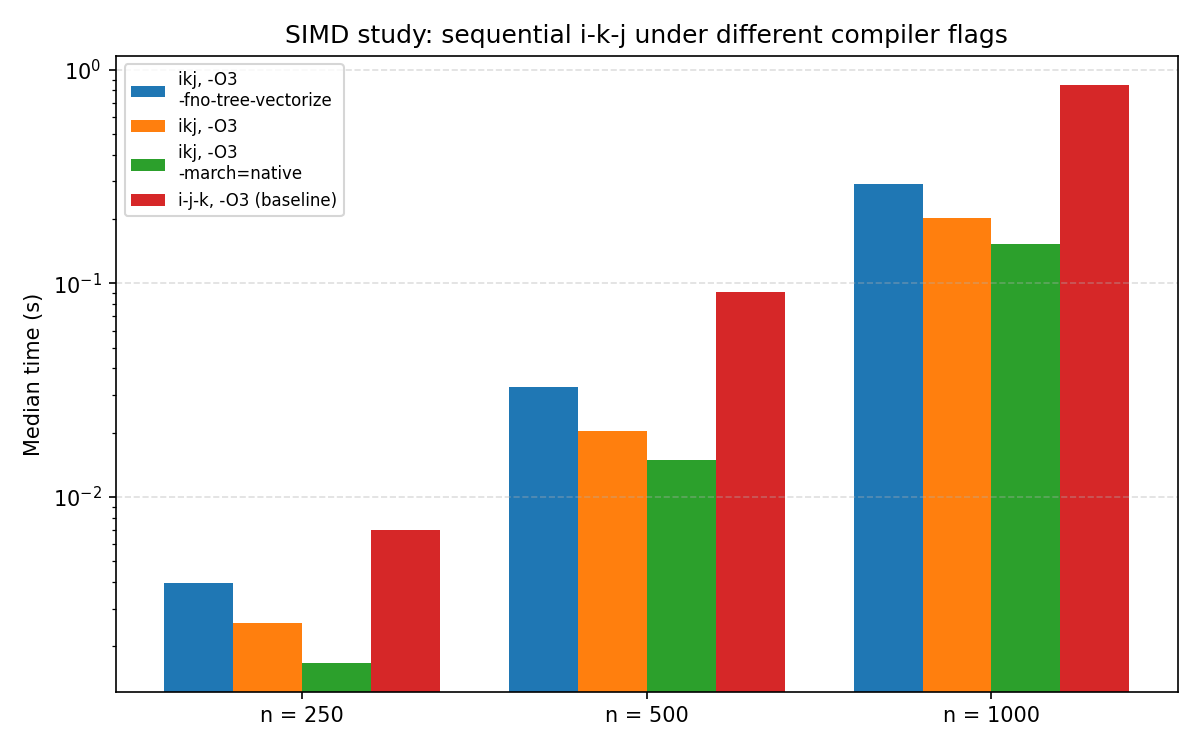
\includegraphics[width=0.9\textwidth]{plot_simd_act3.png}
\caption{SIMD study: median time (log scale) of the i-k-j kernel under
three compiler configurations, compared with the i-j-k \texttt{-O3}
baseline.}
\label{fig:simd}
\end{figure}

\textbf{Analysis:} Table~\ref{tab:simd} and Figure~\ref{fig:simd} evaluate
the optional SIMD extension on the single-threaded i-k-j kernel. Disabling
vectorization (\texttt{-fno-tree-vectorize}) isolates the effect of the loop
reorder alone: it is $2.98\times$ faster than the i-j-k baseline at
$n = 1000$, purely from better data locality. Auto-vectorization
(\texttt{-O3}) then contributes a further $1.55\times$, and
\texttt{-march=native} another $1.19\times$, for a total of $5.47\times$
over the baseline kernel. The compiler report
(\texttt{-fopt-info-vec-optimized}) confirms that the i-k-j innermost loop
is vectorized with 16-byte vectors while the i-j-k innermost loop (a
floating-point reduction) is not, exactly as predicted by dependency
analysis. The vectorization effects are kept strictly separate from the
thread-count effects: all rows of Table~\ref{tab:simd} are single-threaded.

\section{Analysis and discussion}
\label{sec:discussion}

\subsection{Observed performance comparison}
\label{sec:perfcompare}

The experimental results align closely with the architectural
characteristics of the execution environment:
\begin{itemize}
\item \textbf{OpenMP implementation:} Consistently achieves the best
performance for $n \geq 500$, with a practical sweet spot at
$p = 8$--$16$ threads. The maximum speedup obtained was approximately
$5.45\times$ using 22 threads, leading to an efficiency of
$\eta = 5.45 / 22 \approx 25\%$. This behavior aligns with Amdahl's Law:
since a portion of the program is not effectively parallelizable, the
speedup eventually saturates even when increasing threads. Here the
``serial part'' is not literal code --- the kernel has no serial section ---
but synchronization, scheduling and memory-bandwidth contention behave like
one; fitting the observed speedups yields an effective serial-plus-overhead
fraction of roughly 9--15\%.
\item \textbf{Saturation causes:} Two machine-specific effects reinforce the
saturation. The CPU is heterogeneous (only 6 P-cores, so a team of 16--22
threads necessarily includes slower E-core workers), and the working set of
three $1000 \times 1000$ matrices ($\approx$24 MB) exceeds the shared L3, so
concurrent workers compete for memory bandwidth. The fact that $n = 500$
scales slightly better than $n = 1000$ at high $p$ is consistent with a
bandwidth wall: more threads cannot create bandwidth.
\item \textbf{Framework overhead:} OpenMP at $p = 1$ is within 1.4\% of the
sequential baseline, so the fork/join cost is negligible for kernels of this
size.
\item \textbf{Oversubscription:} Running 28 threads on 22 hardware contexts
gives no further benefit in median time ($S = 5.41$) and halves the
efficiency ($E = 0.19$); thread management and context switching absorb the
theoretical gain.
\item \textbf{Threads vs.\ vectorization:} The best parallel configuration
of the baseline i-j-k kernel ($p = 16$: 157.7 ms) and the single-threaded
vectorized i-k-j kernel with \texttt{-march=native} (156.8 ms) are
essentially tied. Each technique buys roughly the same $5.5\times$ on this
workload, but they act on different resources (cores vs.\ vector units), so
they are complementary rather than substitutes. The loop reorder alone ---
before any vector instruction executes --- accounts for $3\times$, a reminder
that ``vectorizable'' often means ``cache-friendly'' at the same time.
\item \textbf{Synchronization:} Synchronization primitives such as locks or
atomics inside the kernel were not required, because each thread computes
independent rows of the resulting matrix with a static schedule: every row
of $\mathbf{C}$ is written by exactly one thread, so no shared write
operations occur, and the parallel result is bit-identical to the sequential
one (maximum elementwise difference exactly zero). If a block-based
parallelization or shared partial accumulators were implemented,
synchronization mechanisms would become necessary to avoid race conditions.
\item \textbf{Resource usage:} The parallel implementations increase memory
access pressure, as multiple threads read rows from $\mathbf{A}$ and
columns from $\mathbf{B}$; in the i-j-k order the innermost loop walks a
column of $\mathbf{B}$ with stride $n$, which is unfavorable for the cache
prefetcher. However, since each thread writes to a distinct row of
$\mathbf{C}$, no write contention occurs. The working set remains
essentially constant across thread counts, so the experiment is limited by
memory bandwidth rather than memory capacity.
\end{itemize}

\subsection{Measurement reliability and environment factors}
\label{sec:reliability}

The methodology incorporated 5 official repetitions preceded by explicit
warm-up phases to minimize cold-start anomalies and transient system noise.
Furthermore, utilizing the median alongside the interquartile range (IQR)
guarantees robustness against isolated outliers caused by background
operating system tasks. The variability is small for the parallel
configurations (IQR below 2\% of the median for $n = 1000$), but the
smallest sizes ($n \leq 250$) have measurement noise comparable to their
runtime and should not be used for scaling conclusions. Thread affinity
could not be controlled on Windows/libgomp, so thread placement is
OS-dependent, and CPU frequency/turbo states were not controlled. Exact
execution times remain strictly bounded by underlying hardware
specifications, CPU clock throttling, and background load. The conclusions
are therefore limited to the configurations actually measured (single
machine, single compiler, $n \leq 1000$, static row partitioning without
cache blocking).

\section{Benchmarking and profiling tools}
\label{sec:tools}

\begin{itemize}
\item \textbf{Used in the project:}
\begin{itemize}
\item \textit{Timing \& Metrics:} \texttt{QueryPerformanceCounter} for
high-resolution wall-clock timing, and the Windows process API
\texttt{GetProcessMemoryInfo} (\texttt{psapi}) for memory tracking in C.
\item \textit{Compilation \& Vectorization evidence:} gcc 16.2.0 with
\texttt{-O3 -fopenmp}, and \texttt{-fopt-info-vec-optimized} to report which
loops were auto-vectorized.
\item \textit{Data Processing \& Visualization:} Python scripts utilizing
\texttt{pandas} for data unification and \texttt{matplotlib} for automated
plot generation and IQR variability computation; \texttt{numpy} as
correctness reference.
\end{itemize}
\item \textbf{Recommended for advanced analysis:}
\begin{itemize}
\item \textit{For C/OpenMP:} Linux \texttt{perf} (cycles, cache misses,
bandwidth counters), Intel VTune Profiler for thread scaling and memory
access analysis, and \texttt{likwid-perfctr} for uncore/memory-bandwidth
counters.
\item \textit{For thread behavior:} \texttt{OMP\_DISPLAY\_ENV} to verify
the real thread configuration, and Extrae/Paraver (or Intel Trace Analyzer)
to visualize thread timelines and imbalance.
\item \textit{For vectorization:} \texttt{llvm-mca} or Intel IACA for
static throughput analysis of the generated inner loops.
\end{itemize}
\end{itemize}

\section{Optimization recommendations}
\label{sec:opt}

To overcome the performance bottlenecks identified during benchmarking,
several optimization strategies can be implemented:
\begin{itemize}
\item \textbf{Algorithmic optimization:} Implement blocked (tiled) matrix
multiplication to significantly improve CPU cache hit rates (L1/L2/L3) and
reduce memory-bandwidth pressure for large matrices; the i-k-j row update is
already the natural kernel for tiling.
\item \textbf{Parallel + SIMD combination:} Combine OpenMP with the
vectorized i-k-j kernel: the two techniques act on different resources
(cores vs.\ vector units) and should multiply their gains.
\item \textbf{Thread management:} Enforce explicit thread affinity (on
platforms where libgomp supports it), study dynamic versus static
scheduling, and repeat the analysis on a homogeneous server CPU to separate
the heterogeneous-core effect from the bandwidth effect.
\item \textbf{Scaling further:} Evaluate larger matrix sizes beyond the
shared L3, and offload to GPU acceleration (e.g., CUDA/OpenCL libraries) if
the bandwidth wall of the host memory is the ultimate limit.
\end{itemize}

\section{Conclusions}
\label{sec:concl}

\begin{itemize}
\item \textbf{Performance findings:} Within the evaluated scope
($n \in \{250, 500, 1000\}$, p $\in \{1, \dots, 28\}$), thread parallelism
delivers up to $5.45\times$ speedup, saturating around $p = 16$--$22$ with
efficiency falling to $0.25$; the practical sweet spot is
$p \in \{8, 16\}$. Oversubscribing the 22 hardware threads brings no
benefit, and the OpenMP overhead at $p = 1$ is negligible ($\approx
1.4\%$).
\item \textbf{Vectorization finding:} A vectorizable i-k-j ordering with
\texttt{-march=native} matches the 16-thread parallel speedup in a single
thread ($5.47\times$ over the i-j-k baseline), confirming that
vectorization and threading are complementary.
\item \textbf{Experimental rigor:} Ensuring reproducible benchmarks
required identical input matrices across methods, warm-up phases, multiple
official repetitions with median/IQR statistics, and checksum validation
against both the sequential reference and NumPy.
\item \textbf{Open limitations:} How the two axes combine (parallel i-k-j),
how the curves shift on a homogeneous server CPU or under enforced
affinity, and how the saturation point moves with $n$ far beyond the
last-level cache remain unresolved.
\item \textbf{AI Collaboration Disclosure:} In accordance with transparent
academic practices, OpenCode (a large-language-model-based CLI assistant)
was utilized during the development of this project. Its purpose was
strictly limited to assisting with technical writing, structuring the
academic report in LaTeX, debugging compilation errors, and refining the
data analysis methodology. All benchmarking executions, code
implementations, and final validations were independently performed and
verified by the author, who also generated all figures locally and checked
every reported number against the raw CSV measurements.
\end{itemize}

\end{document}
